\documentclass{article}
% translate with >> pdflatex -shell-escape <file>

% This file is an extract of the PGFPLOTS manual, copyright by Christian Feuersaenger.
% 
% Feel free to use it as long as you cite the pgfplots manual properly.
%
% See
%   http://pgfplots.sourceforge.net/pgfplots.pdf
% for the complete manual.
%
% Any required input files (for <plot table> or <plot file> or the table package) can be downloaded
% at
% http://www.ctan.org/tex-archive/graphics/pgf/contrib/pgfplots/doc/latex/
% and
% http://www.ctan.org/tex-archive/graphics/pgf/contrib/pgfplots/doc/latex/plotdata/

\usepackage{pgfplots}
\pgfplotsset{compat=newest}

\pagestyle{empty}

\begin{document}
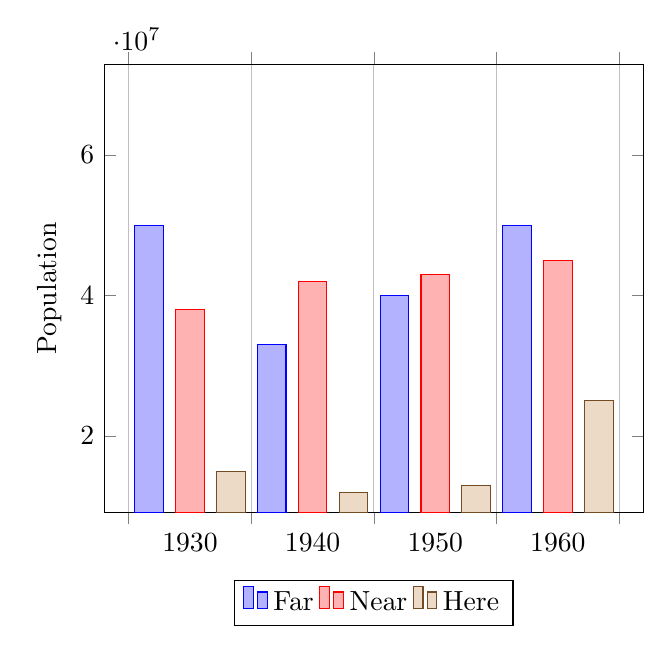
\begin{tikzpicture}
\begin{axis}[
	x tick label style={
		/pgf/number format/1000 sep=},
	ylabel=Population,
	enlargelimits=0.05,
	legend style={at={(0.5,-0.15)},
		anchor=north,legend columns=-1},
	ybar interval=0.7,
]
\addplot 
	coordinates {(1930,50e6) (1940,33e6)
		 (1950,40e6) (1960,50e6) (1970,70e6)};

\addplot 
	coordinates {(1930,38e6) (1940,42e6) 
		(1950,43e6) (1960,45e6) (1970,65e6)};

\addplot 
	coordinates {(1930,15e6) (1940,12e6) 
		(1950,13e6) (1960,25e6) (1970,35e6)};
\legend{Far,Near,Here}
\end{axis}
\end{tikzpicture}
\end{document}
